\begin{enumerate}
    \item  Bellmam Equation $$v(k_t)= max_{k_{t+1}} \frac{(k_t^\theta -k_{t+1}+(1-\delta)k_t)^{1-\sigma}-1}{1-\sigma}+\beta v(k_{t+1})$$\\
    FOC: please note $x_t=k_t, y_t=k_{t+1}$ please also note that $x_{s+1}=G(x_s,y_s)$
    
    $$\frac{\partial v(k_t)}{\partial k_{t+1}}=-( -k_{t+1} + (1-\delta)*k_t +k_t^\theta)^{-\sigma}
   +\beta v'(G(x_t,y_t))*G_{x_t}(x_{t+1},y_{t+1})$$
   non zero steady state 
   $$$$
   \item. 
   \item
   \begin{figure}[h]
       \centering
       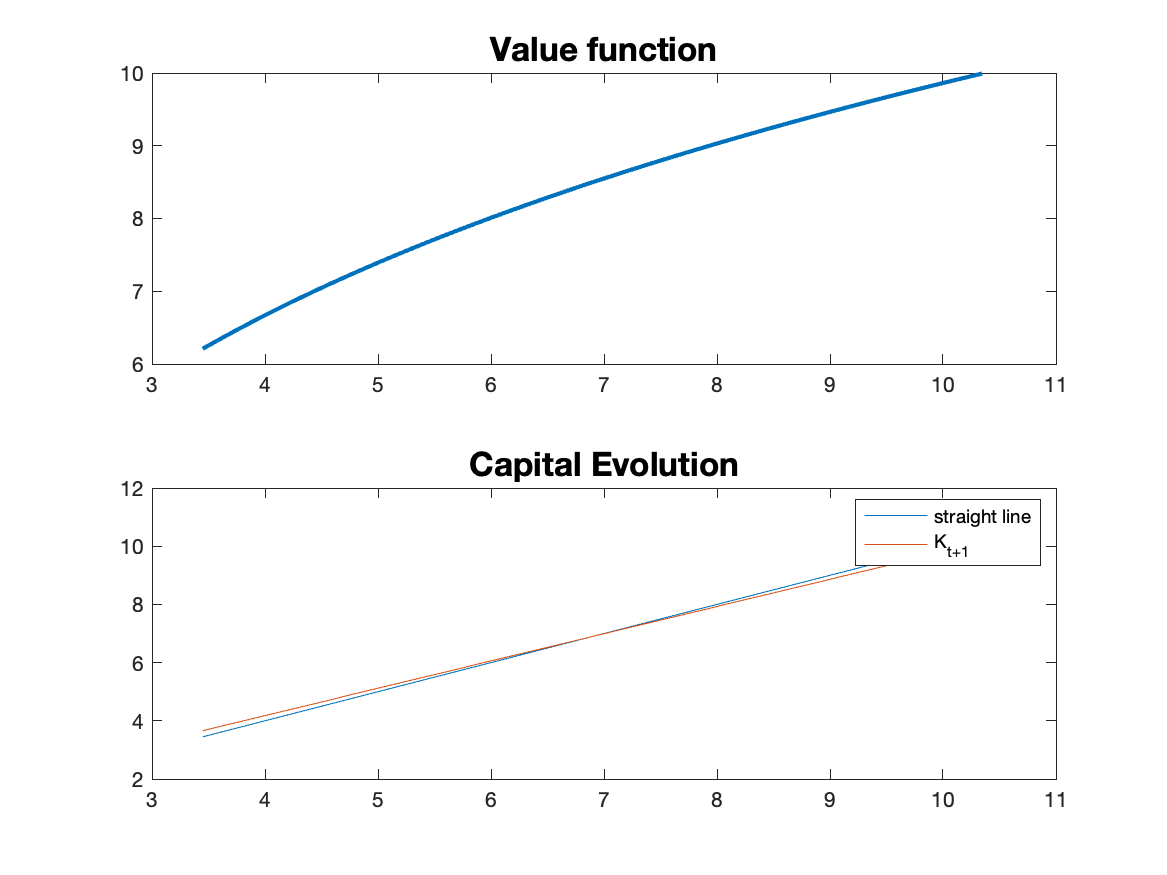
\includegraphics[width = .8\linewidth]{HW3/pics/HW3_Q2_figure.png}
       \caption{The steady state equilibrium would be stable as the $k_{t+1}$ function is above the 45 degree line before the steady state and below the 45 degree line after the steady state}
       \label{fig:my_label}
   \end{figure}
\end{enumerate}